\documentclass{cskkuproject}

% ==========================================
% ข้อมูลโครงงาน — กรอกข้อมูลที่นี่
% ==========================================

\titleTH{ระบบแนะนำสินค้าเชิงสนทนาด้วยปัญญาประดิษฐ์}
\titleEN{AI-Based Conversational Product Recommendation System}

% ข้อมูลนักศึกษาคนที่ 1
\firstStudentID{663380236-4}
\firstStudentPrefixTH{นาย}
\firstStudentPrefixEN{Mr.}
\firstStudentNameTH{ศจิษฐา ศีลธรรมดี}
\firstStudentNameEN{Sachittha Sinthamdi}

% ข้อมูลนักศึกษาคนที่ 2
% *** ถ้าทำโครงงานคนเดียว ให้เว้นว่างไว้ทั้งหมด (เหมือนด้านล่าง) ***
% *** ถ้ามี 2 คน ให้กรอกข้อมูลเหมือนคนที่ 1 ***
\secondStudentID{663380215-2}
\secondStudentPrefixTH{นาย}
\secondStudentPrefixEN{Mr.}
\secondStudentNameTH{นิติธร คชรัตน์}
\secondStudentNameEN{Nititorn Khotcharat}

% ข้อมูลหลักสูตร
\degreeTH{วิทยาศาสตรบัณฑิต}
\degreeEN{Bachelor of Science}
\majorTH{วิทยาการคอมพิวเตอร์}
\majorEN{Computer Science}

% อาจารย์ที่ปรึกษา
\advisorTH{อ.ดร.พงษ์ศธร จันทร์ยอย}
\advisorEN{Pongsathorn Chanyoy, Ph.D.}

% ปีการศึกษา
\academicYearTH{2569}
\academicYearEN{2026}

% รหัสวิชา (CP354 771 = โครงงาน 1, CP354 772 = โครงงาน 2)
\courseCode{CP354 771}
\courseName{โครงงานคอมพิวเตอร์ 1}
\semester{1}

% คำสำคัญ
\keywordsTH{ระบบแนะนำสินค้าเชิงสนทนา, การสร้างคำตอบโดยอาศัยการค้นคืน, เอเจนต์อัจฉริยะ, การค้นคืนข้ามภาษา, แบบจำลองภาษาขนาดใหญ่}
\keywordsEN{Conversational Recommender System, Retrieval-Augmented Generation, Agentic RAG, Cross-lingual Retrieval, Large Language Model}



% ==========================================
% ปรับเฉพาะบรรทัดหัวเรื่องของหน้าปก
% เลย์เอาต์คงเดิมทุกอย่างตามคลาสของคณะ
% เปลี่ยนเป็น "ฉบับสมบูรณ์" เมื่อส่งเล่มจบ
% ==========================================
\makeatletter
\renewcommand{\maketitlepage}{
\begin{titlepage}
\clearpage
\thispagestyle{empty}
\centering


\includegraphics[scale=0.5]{./theme/kku-logo.png}

{\Large\bfseries เอกสารโครงงานฉบับความก้าวหน้า ครั้งที่ 2}

\vfill

{\Large \@titleTH \\[0.5cm] \@titleEN}

\vfill

{\large โดย \\}
{\large \@firstStudentID~\@firstStudentPrefixTH\@firstStudentNameTH \\}
\IfEmptyTF{\@secondStudentID}{}{%
  {\large \@secondStudentID~\@secondStudentPrefixTH\@secondStudentNameTH \\}%
}
\vspace{1cm}

{\large อาจารย์ที่ปรึกษา \\ \@advisorTH \\}

\vfill

{\large รายงานฉบับนี้เป็นส่วนหนึ่งของการศึกษา\\}
{\large วิชา \@courseCode{} \@courseName\\}
{\large หลักสูตร\@degreeTH{} สาขาวิชา\@majorTH\\}
{\large วิทยาลัยการคอมพิวเตอร์\\}
{\large มหาวิทยาลัยขอนแก่น\\}
{\large ปีการศึกษา \@academicYearTH}

\end{titlepage}
}
\makeatother


\begin{document}

% ==========================================
% หน้าปก
% ==========================================
% คำสั่งด้านล่างสร้างหน้าปกอัตโนมัติจากข้อมูลที่กรอกด้านบน
% ไม่ต้องแก้ไขส่วนนี้
\maketitlepage

% ตั้งค่าเลขหน้าส่วนต้นเป็นอักษรไทย (ก, ข, ค, ...)
\pagenumbering{arabic}
\setcounter{page}{0}
\renewcommand{\thepage}{\ThaiAlph{\value{page}}}

% ==========================================
% บทคัดย่อ
% ==========================================
\begin{abstractTH}
% บทคัดย่อภาษาไทย — ไม่เกิน 300 คำ
% ครอบคลุม: วัตถุประสงค์ → วิธีการ → ผลลัพธ์ → การประยุกต์ใช้

โครงงานนี้มีวัตถุประสงค์เพื่อเปรียบเทียบสถาปัตยกรรมการสร้างคำตอบโดยอาศัยการค้นคืนแบบมาตรฐานกับแบบที่มีเอเจนต์ตัดสินใจเอง บนระบบแนะนำสินค้าเชิงสนทนาที่รับคำถามได้ทั้งภาษาไทยและภาษาอังกฤษ โดยคลังสินค้าเป็นภาษาอังกฤษทั้งหมด

วิธีดำเนินงานเริ่มจากเตรียมคลังสินค้าจริงจาก Amazon จำนวน 81{,}264 รายการ สร้างดัชนีค้นหาเชิงความหมายด้วยแบบจำลองฝังเวกเตอร์สองภาษา แล้วพัฒนาสถาปัตยกรรม 3 แบบที่ใช้ส่วนประกอบร่วมกันทั้งหมดและต่างกันเฉพาะชั้นที่แบบจำลองภาษาตัดสินใจเอง เพื่อให้การเปรียบเทียบเปลี่ยนตัวแปรทีละตัว ระบบทั้งหมดประมวลผลบนเครื่องคอมพิวเตอร์ส่วนบุคคลด้วยแบบจำลองภาษาขนาด 8 พันล้านพารามิเตอร์ การประเมินใช้ชุดทดสอบที่สร้างขึ้นเอง 140 คำค้นสองภาษา แบ่งตามสิ่งที่คลังมี และติดเฉลยความตรงด้วยมือตามเกณฑ์มาตรฐาน 4 ระดับ

ผลการทดลองพบว่าสถาปัตยกรรมแบบเอเจนต์ให้คะแนน nDCG@3 สูงกว่าแบบมาตรฐานทั้งสองภาษาและไม่แพ้แม้แต่คำค้นเดียว โดยฝั่งอังกฤษเพิ่มจาก 0.3288 เป็น 0.3564 อย่างมีนัยสำคัญทางสถิติ และฝั่งไทยเพิ่มจาก 0.3165 เป็น 0.3267 อย่างไรก็ตาม ความได้เปรียบทั้งหมดมาจากกลุ่มคำค้นที่คลังไม่มีสินค้าตรงเท่านั้น ส่วนกลุ่มที่คลังมีสินค้าตรงนั้นทุกสถาปัตยกรรมได้คะแนนเท่ากัน นอกจากนี้ยังพบว่าชั้นจัดอันดับเป็นคอขวดที่แท้จริงของระบบ เนื่องจากทำให้สินค้าที่ตรงสูญหายไปร้อยละ 45 ถึง 48 ซึ่งมากกว่าทุกชั้นอื่นรวมกันประมาณ 3.5 เท่า และการเพิ่มสัญญาณนับคำที่ซ้อนกับคำค้นเข้าไปในชั้นนี้ให้ผลดีกว่าการเพิ่มความเป็นเอเจนต์ประมาณ 2 เท่า

ผลที่ได้นำไปใช้เป็นแนวทางเลือกสถาปัตยกรรมสำหรับระบบค้นหาสินค้าได้ คือความเป็นเอเจนต์คุ้มค่าเมื่อคำค้นมีโอกาสหาของไม่เจอ ไม่ใช่ทุกกรณี และโครงงานนี้ได้เผยแพร่ชุดทดสอบพร้อมเฉลยสู่สาธารณะเพื่อให้ผู้อื่นนำไปวัดผลซ้ำได้

\end{abstractTH}

\begin{abstractEN}
% ABSTRACT (English) — should not exceed 300 words
% Past tense for objectives and methodology
% Present tense for results and applications

This project aimed to compare a standard retrieval-augmented generation architecture with an agentic one, in which a language model makes decisions at run time, for a conversational product recommendation system that accepts queries in both Thai and English over an English-only product catalogue.

The work began by preparing a real catalogue of 81{,}264 Amazon products and building a semantic search index with a bilingual embedding model. Three architectures were then developed. All of them share every component and differ only in which layers the language model decides for itself, so that the comparison changes one variable at a time. The entire system runs on a personal computer using an 8-billion-parameter language model, without calling any external service. Evaluation used a purpose-built test collection of 140 queries in both languages, grouped by what the catalogue actually contains, with relevance judgements assigned by hand following a standard four-level scheme.

The results show that the agentic architectures score higher than the standard one in both languages and lose on no query at all. The English score rises from 0.3288 to 0.3564, which is statistically significant, and the Thai score rises from 0.3165 to 0.3267. However, the entire advantage comes from queries for which the catalogue holds no matching product. When the catalogue does hold a match, all three architectures score identically. The study further finds that the ranking layer, not the retrieval or decision layer, is the real bottleneck: it loses 45 to 48 percent of the relevant products, roughly three and a half times more than every other stage combined. Adding a word-overlap signal to that layer yields about twice the gain that the agentic behaviour provides.

These findings give practical guidance for architecture selection, and the test collection with its judgements is released publicly so that others can reproduce the measurements.

\end{abstractEN}

% ==========================================
% กิตติกรรมประกาศ
% ==========================================
\begin{acknowledgement}
% กิตติกรรมประกาศ — ไม่เกิน 1 หน้ากระดาษ

ข้าพเจ้าขอขอบพระคุณ อาจารย์ที่ปรึกษาโครงงาน
ที่ได้กรุณาให้คำแนะนำ คำปรึกษา และข้อเสนอแนะอันเป็นประโยชน์
ตลอดระยะเวลาการดำเนินโครงงานฉบับนี้
โดยเฉพาะข้อเสนอแนะเรื่องการออกแบบการเปรียบเทียบให้เปลี่ยนตัวแปรทีละตัว
ซึ่งเป็นจุดที่ทำให้ข้อสรุปของโครงงานมีความหมาย
รวมทั้งสละเวลาในการตรวจแก้ไขและให้กำลังใจ
จนทำให้โครงงานนี้สำเร็จลุล่วงไปได้ด้วยดี

ขอขอบพระคุณคณาจารย์ในสาขาวิชาวิทยาการคอมพิวเตอร์
วิทยาลัยการคอมพิวเตอร์ มหาวิทยาลัยขอนแก่น
ทุกท่านที่ได้ถ่ายทอดความรู้ทางวิชาการ
ซึ่งเป็นพื้นฐานสำคัญในการศึกษาค้นคว้าและจัดทำโครงงานนี้

ขอขอบคุณผู้จัดทำชุดข้อมูลสาธารณะที่โครงงานนี้นำมาใช้
ทั้งชุดข้อมูลสินค้าและชุดคำค้นมาตรฐาน
ซึ่งทำให้การประเมินผลตั้งอยู่บนข้อมูลจริงของผู้ใช้
แทนที่จะเป็นข้อมูลที่สร้างขึ้นเอง

ขอขอบคุณเพื่อนร่วมชั้นและผู้ที่เกี่ยวข้องทุกท่าน
ที่ได้ให้ความช่วยเหลือ แนะนำ และแลกเปลี่ยนความคิดเห็น
ซึ่งเป็นประโยชน์ต่อการดำเนินงานในหลายด้าน

ท้ายที่สุดนี้ ข้าพเจ้าขอขอบพระคุณบิดา มารดา และครอบครัว
ที่ให้การสนับสนุน ส่งเสริม และเป็นกำลังใจ
ตลอดระยะเวลาของการศึกษา

\end{acknowledgement}

% ==========================================
% สารบัญ
% ==========================================
\tableofcontents
\clearpage
\listoffigures
\clearpage
\listoftables
\clearpage

% ==========================================
% สัญลักษณ์และคำย่อ (ถ้ามี — uncomment ด้านล่าง)
% ==========================================
% \begin{symbolpage}
% \input{symbols}
% \end{symbolpage}

% ==========================================
% เนื้อเรื่อง 5 บท
% ==========================================
% เริ่มนับเลขหน้าใหม่เป็นเลขอารบิก (1, 2, 3, ...)
% ไม่ต้องแก้ไขส่วนนี้
\pagenumbering{arabic}
\setcounter{page}{1}

\chapterone
\chaptertwo
\chapterthree
\chapterfour
\chapterfive

% ==========================================
% เอกสารอ้างอิง
% ==========================================
% *** ไม่ต้องแก้ไขส่วนนี้ ***
% ระบบจะดึงรายการอ้างอิงจากไฟล์ references.bib อัตโนมัติ
% ให้แก้ไขรายการอ้างอิงในไฟล์ references.bib แทน
\clearpage
\addcontentsline{toc}{chapter}{เอกสารอ้างอิง}
\makeatletter
\let\ps@plain\ps@empty
\makeatother
\bibliographystyle{ieeetr}
\bibliography{references}

% ==========================================
% ภาคผนวก
% ==========================================
% =============================
% ภาคผนวก
% =============================
% ใช้คำสั่ง \appendiceschapter{ชื่อภาคผนวก} สำหรับแต่ละภาคผนวก
% ระบบกำหนดตัวอักษร ก, ข, ค ... ให้เอง

% =============================
% ภาคผนวก ก
% =============================
\setcounter{chapter}{-1}
\appendiceschapter{หน้าจอสาธิตระบบ}

\section*{ภาพรวมของหน้าจอสาธิต}

โครงงานนี้พัฒนาหน้าจอสาธิตขึ้นเพื่อให้ทดลองใช้ระบบได้จริง และเพื่อให้เห็นความต่าง
ระหว่างสถาปัตยกรรมทั้งสามแบบขณะทำงาน หน้าจอนี้ทำงานบนเครื่องส่วนบุคคลเช่นเดียวกับ
ตัวระบบ และเรียกใช้สถาปัตยกรรมตัวจริงชุดเดียวกับที่ใช้วัดผลในบทที่ 4
ไม่ได้แสดงผลลัพธ์ที่เตรียมไว้ล่วงหน้า

หน้าจอหลักก่อนเริ่มถามคำถามแสดงดังภาพที่ \ref{fig:demo_ui}

\begin{figure}[H]
\centering
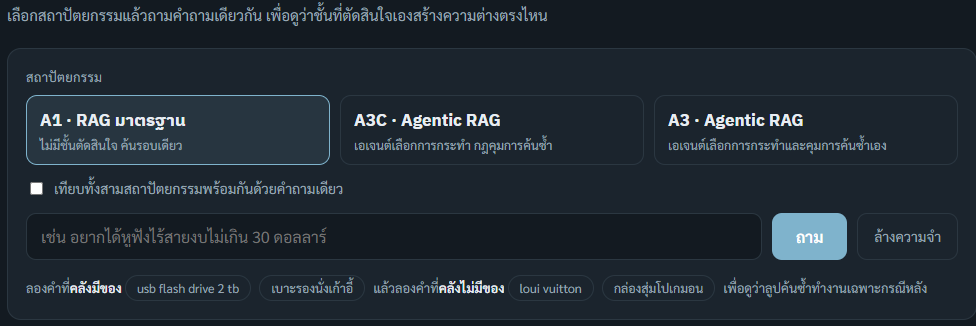
\includegraphics[width=\textwidth]{images/demo-ui.png}
\caption{หน้าจอหลักของระบบสาธิต ส่วนเลือกสถาปัตยกรรมและช่องพิมพ์คำถาม}
\label{fig:demo_ui}
\end{figure}

ส่วนประกอบของหน้าจอแบ่งเป็น 4 ส่วน ดังนี้

\begin{enumerate}[label=\arabic*)]
    \item \textbf{ส่วนเลือกสถาปัตยกรรม} ผู้ใช้เลือกได้ว่าจะให้คำถามนี้ทำงานด้วย A1 ซึ่งเป็น
          RAG มาตรฐาน A3C ซึ่งเป็น Agentic RAG ที่เอเจนต์เลือกการกระทำ หรือ A3
          ซึ่งเอเจนต์คุมการค้นซ้ำเองด้วย ใต้ชื่อแต่ละแบบมีคำอธิบายสั้นกำกับว่าต่างกันอย่างไร
    \item \textbf{ตัวเลือกเทียบทั้งสามแบบพร้อมกัน} เมื่อเปิดใช้ ระบบจะส่งคำถามเดียวกัน
          ไปยังทั้งสามสถาปัตยกรรมแล้วแสดงผลเรียงลงมา ทำให้เปรียบเทียบได้ในคราวเดียว
    \item \textbf{ช่องพิมพ์คำถาม} รับได้ทั้งภาษาไทยและภาษาอังกฤษ ระบบตรวจภาษาเองแล้วตอบ
          เป็นภาษาเดียวกับที่ถาม ข้างล่างมีคำค้นตัวอย่างที่กดใช้ได้ทันที
          แบ่งเป็นกลุ่มที่คลังมีสินค้าและกลุ่มที่คลังไม่มีสินค้า
    \item \textbf{ปุ่มล้างความจำ} เนื่องจากแต่ละสถาปัตยกรรมจดจำบทสนทนาข้ามรอบ
          การเริ่มคำถามใหม่ที่ไม่เกี่ยวกับคำถามก่อนจึงต้องล้างความจำก่อน
\end{enumerate}

\section*{ผลการเปรียบเทียบสามสถาปัตยกรรมด้วยคำถามเดียวกัน}

ภาพที่ \ref{fig:demo_compare} แสดงผลเมื่อเปิดโหมดเทียบทั้งสามแบบ แล้วถามด้วยคำค้น
\texttt{loui vuitton} ซึ่งเป็นคำค้นจริงจากชุดทดสอบในกลุ่มที่คลังไม่มีสินค้าตรง
และเป็นคำที่ผู้ใช้สะกดผิดจากคำว่า louis vuitton

\begin{figure}[H]
\centering
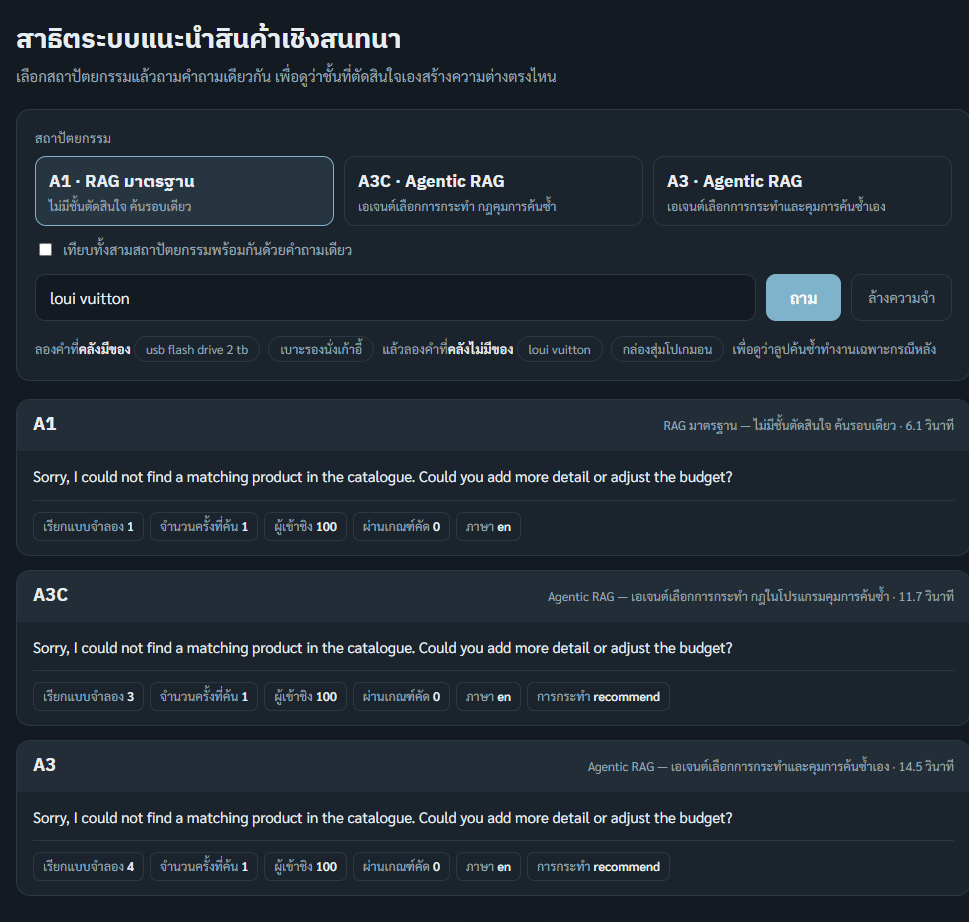
\includegraphics[width=\textwidth]{images/demo-compare.png}
\caption{ผลการเปรียบเทียบทั้งสามสถาปัตยกรรมด้วยคำถามเดียวกัน}
\label{fig:demo_compare}
\end{figure}

\subsection*{การอ่านผลในภาพ}

ใต้คำตอบของแต่ละสถาปัตยกรรมมีแถบตัวเลขที่ดึงมาจากการทำงานจริงของรอบนั้น
ได้แก่ จำนวนครั้งที่เรียกแบบจำลองภาษา จำนวนครั้งที่ค้น จำนวนผู้เข้าชิงที่ดึงมาจากคลัง
จำนวนที่ผ่านเกณฑ์คัด ภาษาที่ตรวจได้ และการกระทำที่ชั้นวางแผนเลือก
สรุปค่าที่ปรากฏในภาพได้ดังตารางที่ \ref{tab:demo_trace}

\begin{table}[H]
\centering
\caption{ค่าที่วัดได้จากหน้าจอสาธิตในภาพที่ \ref{fig:demo_compare}}
\label{tab:demo_trace}
\begin{tabular}{|l|c|c|c|}
\hline
\textbf{รายการ} & \textbf{A1} & \textbf{A3C} & \textbf{A3} \\
\hline
เรียกแบบจำลองภาษา (ครั้ง) & \textbf{1} & 3 & 4 \\ \hline
จำนวนครั้งที่ค้น & 1 & 1 & 1 \\ \hline
ผู้เข้าชิงที่ดึงจากคลัง & 100 & 100 & 100 \\ \hline
ผ่านเกณฑ์คัด & 0 & 0 & 0 \\ \hline
เวลาที่ใช้ (วินาที) & \textbf{6.1} & 11.7 & 14.5 \\ \hline
คำตอบ & ไม่พบ & ไม่พบ & ไม่พบ \\
\hline
\end{tabular}
\end{table}

สิ่งที่ภาพนี้แสดงมี 3 ประการ

\begin{enumerate}[label=\arabic*)]
    \item \textbf{ทั้งสามสถาปัตยกรรมปฏิเสธถูกต้องตรงกัน} เนื่องจากไม่มีสินค้าใด
          ผ่านเกณฑ์คัดเลยแม้แต่ชิ้นเดียว ระบบจึงตอบว่าไม่พบแทนที่จะเสนอสินค้าที่ไม่ตรง
          ซึ่งเป็นพฤติกรรมที่ถูกต้องสำหรับคำค้นกลุ่มนี้
    \item \textbf{ต้นทุนเพิ่มขึ้นตามความเป็นเอเจนต์ แต่ผลลัพธ์เท่ากัน} A1 เรียกแบบจำลอง
          เพียงครั้งเดียวและใช้เวลา 6.1 วินาที ขณะที่ A3 เรียก 4 ครั้งและใช้เวลา 14.5 วินาที
          หรือราว 2.4 เท่า ทั้งที่ได้คำตอบเหมือนกันทุกประการ
          ข้อสังเกตนี้สอดคล้องกับข้อสรุปในบทที่ 5 ที่ว่าการขยายขอบเขตการตัดสินใจของ
          เอเจนต์ไปถึงการคุมการค้นซ้ำนั้นไม่คุ้มกับต้นทุนที่เพิ่มขึ้น
    \item \textbf{ชั้นวางแผนทำงานจริง} A3C และ A3 แสดงการกระทำที่เลือกไว้ว่า recommend
          ขณะที่ A1 ไม่มีช่องนี้เพราะไม่มีชั้นวางแผน จึงค้นทันทีทุกครั้ง
\end{enumerate}

\subsection*{ข้อสังเกตเรื่องความจำกับการสาธิต}

ในภาพที่ \ref{fig:demo_compare} จำนวนครั้งที่ค้นของทั้งสามสถาปัตยกรรมเท่ากับ 1
กล่าวคือ\textbf{การค้นซ้ำไม่ได้ทำงาน} ทั้งที่คำค้นนี้อยู่ในกลุ่มที่คลังไม่มีสินค้า
สาเหตุคือรอบนั้นได้ถามคำถามเดียวกันไปก่อนหน้าแล้ว ระบบจึงจดจำไว้ว่าเคยพยายามค้นด้วย
คำนี้แล้วไม่พบ และไม่พยายามซ้ำอีก

เมื่อล้างความจำแล้วถามใหม่ด้วยคำเดียวกัน การค้นซ้ำทำงานตามที่ออกแบบไว้ คือค้น 2 รอบ
และเรียกแบบจำลองภาษา 4 ครั้งสำหรับ A3C โดยคำค้นที่ระบบเขียนขึ้นใหม่ในรอบที่สองคือ
louis vuitton ซึ่งเป็นการแก้คำสะกดจาก loui vuitton ได้ถูกต้อง
กรณีนี้สำเร็จเพราะเป็นชื่อแบรนด์ที่แบบจำลองรู้จัก ไม่ใช่ความสามารถแก้คำสะกดทั่วไป
ตามที่อธิบายไว้ในบทที่ 4

ข้อสังเกตนี้มีผลเชิงปฏิบัติคือ \textbf{การสาธิตควรล้างความจำก่อนเริ่มคำถามใหม่ทุกครั้ง}
มิฉะนั้นพฤติกรรมการค้นซ้ำจะไม่ปรากฏให้เห็น

\section*{วิธีเรียกใช้งาน}

ระบบสาธิตต้องเปิดบริการแบบจำลองภาษาในเครื่องก่อน แล้วจึงเปิดเซิร์ฟเวอร์ของหน้าจอสาธิต
จากนั้นเข้าใช้งานผ่านเว็บเบราว์เซอร์ที่ที่อยู่ภายในเครื่อง
เซิร์ฟเวอร์เขียนด้วยไลบรารีมาตรฐานของภาษาไพทอนทั้งหมด จึงไม่ต้องติดตั้งเว็บเฟรมเวิร์กเพิ่ม


% ==========================================
% ประวัติผู้เขียน
% ==========================================
\begin{biography}
% ประวัติผู้เขียน — ไม่เกิน 1 หน้ากระดาษ

\section*{นักศึกษาคนที่ 1}

นายศจิษฐา ศีลธรรมดี เกิดเมื่อวันที่ 3 กันยายน พ.ศ. 2547
สำเร็จการศึกษาระดับมัธยมศึกษาตอนปลาย จากโรงเรียนราชสีมาวิทยาลัย เมื่อปีการศึกษา 2565
ปัจจุบันกำลังศึกษาระดับปริญญาตรี หลักสูตรวิทยาศาสตรบัณฑิต
สาขาวิชาวิทยาการคอมพิวเตอร์ วิทยาลัยการคอมพิวเตอร์ มหาวิทยาลัยขอนแก่น

\section*{นักศึกษาคนที่ 2}

นายนิติธร คชรัตน์ เกิดเมื่อวันที่ 22 มิถุนายน พ.ศ. 2547
สำเร็จการศึกษาระดับมัธยมศึกษาตอนปลาย จากโรงเรียนแก่นนครวิทยาลัย เมื่อปีการศึกษา 2565
ปัจจุบันกำลังศึกษาระดับปริญญาตรี หลักสูตรวิทยาศาสตรบัณฑิต
สาขาวิชาวิทยาการคอมพิวเตอร์ วิทยาลัยการคอมพิวเตอร์ มหาวิทยาลัยขอนแก่น

\end{biography}

\end{document}
